\section{itération 1 : nouveau BS au standard MQTT}
        \gls{mdi}, étant une entreprise innovante en télématique, doit toujours
        suivre et avancer les nouvelles technologies. Une de ces technologies
        est le protocol de communication standard des objets connectés: le MQTT.

        ...
        


    \subsection{Descriptif du protocole:Le standard MQTT, l'essentiel à savoir}
    D’apres la specification officielle MQTT \cite{mqtt_site},
    le standard MQTT est un protocole de transport de message Client/serveur sous le pattern de Publication/Souscription 
    “ Publish/ Subscribe”. 
    C'est un protocole léger , ouvert, simple et désigné d’être facile à implémenter. \\
    Ces caractéristiques le rend idéal à être utilisé dans plusieurs situations, surtout pour la communication Machine 
    to MAchine M2M et pour l’internet des objets IoT. Des contextes où la faible empreinte du code est requise ainsi 
    qu’une bonne bande passante.     \\
    
    {
        \large 
        \centering
        \textbf{Qu’offre MQTT ? }\\
    
    }   
   
    \begin{itemize}
        \renewcommand{\labelitemi}{$\bullet$}
        \item L’utilisation du pattern de message “ Publication/Souscription” qui offre 
        des distributions un-à-plusieurs ( one-to-many) et le découplage de ces deux parties.    
        \item 3 Qualités de service QoS pour la distribution des messages . 
        \item Un échange de protocol minimisé pour réduire le trafic  du réseau      
        \item Un mécanisme pour notifier les parties intéressées lors d'une déconnexion anormal    
    \end{itemize}   
    \bigskip 
    En cas de besoin de plus de détails sur le standard, consultez la partie Annexes. Elle comporte des eclaicissements 
    sur le standard MQTT.\\

    {
        \large 
        \centering
        \textbf{En quoi MQTT sera meilleur ?  } 
    
    }  
    Pour répondre à une telle question il faut comparer entre MQTT et le protocole de \gls{mdi21} comme le montre le tableau \ref{table:mqttvsmd21}
    de la page \pageref{table:mqttvsmd21}.
    \begin{table}[h!]
        \centering
        \begin{tabular}{|p{5cm}|p{5cm}|p{5cm}|}
            \hline
            \centering

               & MQTT & \gls{mdi21} \\
            \hline
            Logique & standardisée & fait maison  \\
            \hline
           Protocole basé sur & TCP/IP & TCP - UDP\\
            \hline 
            Couplage entre BS et consommateurs & Broker découplé des consommateurs & couplage fort \\
            \hline
        \end{tabular}   
        \caption{Tableau de comparaison : MQTT vs MD21}
        \label{table:mqttvsmd21}
    \end{table} \\
       

        Cette compariaosn montre les différences entre les deux protocoles en mettant en valeur les points considérés forts de MQTT par rapport
        à \gls{mdi21}. 
        Ces points sont autour la logique du protocole adapté, leurs protcoles de base et le degrée de couplage avec les consomatteurs 
        ou la partie traitement dans notre cas. \\
        
    \subsection{Specifications techniques \& Implémentation}
       
        Le Point d’entrée du cloud ou BS se charge de deux principales fonctionnalités. 
        \begin{itemize}
            \renewcommand{\labelitemi}{$\bullet$}
            \item  \textbf{Transfert de données :} où ils gèrent les connexions avec les boîtiers.
            \item  \textbf{Traitement de données :} encodage/décodage des données de messages selon le format de données du cloud.
        \end{itemize}

        Puisque le standard repose sur le découplage entre le publisher et subscriber, la conception doit prendre 
        en compte  un broker MQTT pour assurer cette notion. 
        La conception est présenté par la figure suivante .. 

 ********* Insertion d une figure de la conception ************** \\
        Le BS aura deux parties importantes qui sont le transfert des données et l'encodage pour le broker.

    \subsubsection{Recherche \& état de l'art}
            

        Il existe quelque large implémentation de MQTT comme Facebook Messenger par example, mais aussi de nombreux 
        outils monétisés et d'autres open source.
        Il y a aussi un projet Eclipse active, "Paho", qui offre une implémentation scalable , open source pour 
        différents langage de programmation comme Java , 
        C, C++ , Python , JavaScript , C\# et Go lang. \\
        Il existe plusieurs implémentations qui sont réunis dans cette référance \cite{mqtt_choix} publié par un des membbre de la communauté de MQTT et qui les comparent selon plusieurs critères. 
        Pour effectuer un bon choix satisfaisant de toute ce    s propositions, il faut bien demander les critères de l'entreprise en premier lieu 
        sur lesquels on se base. \\
        
        {\centering
        \Large
        \textbf{A la recherche d'un broker MQTT! } \\}
        \vspace{0.2cm}
        Comme la stratégie de l entreprise est de réduire les coûts, nous éliminons les choix d'outils payants. \\
        D'autre part, le support de QoS 2 n'est pas exigé vue que l'échange de message en QoS 2 est trés couteux. 
        Tandis que le QoS 1 est indispensable pour profiter du système des ack.\\
        Un autre critère est la charge des connexions du broker. L'un des objectifs de \gls{md30} est d'augmenter le support 
        en charge du nouveau BS ce qui revient dans ce cas à étudier la charge du broker MQTT en question. 
        Ceci peut être effectué de deux manières : 
        \begin{itemize}
            \item Augmenter le support en charge du Broker par rapport au \gls{BS} de \gls{mdi21}, sachant que
            le support du BS actuel est de ... 
            \item Assurer la scalabilité du broker ce qui revient à choisir dés le début un broker scalable.
        \end{itemize} 
        \vspace{0.3cm}
        En se basant sur ces critères, nous éliminons déjà beaucoup de choix pour rester avec les implémentations des projets 
        open source qui ont implémenté la QoS 1 ainsi qu'une solution pour la sclalabilité du broker. En plus il faut que le projet soit mis 
        à jour avec une communauté qui le supporte.  
        Nous nous retrouvons alors avec 2 choix qui répondent à nos critères : 
        \begin{itemize}
            \item HmQ : Broker MQTT open source développé en Go lang. 
            \item Mosca : Broker MQTT open source déeloppé en Node.JS. 
        \end{itemize} 
        
        Afin de déterminer lequel de ces brokers sera choisi il faut bien vérifier qu il répondent aux attentes en effectuons quelques tests. 
        Pour ce faire nous avons intégrés les brokers dans la chaine de transfert des données jusqu' à lentrée dans le cloud - 
        c'est à dire le push dans kafka.


        \subsubsection{Développement effectué}

        L'intégration du broker dans la chiane de push qui est composé par:\\
         . Traitement de données:
            le(s) subscriber(s) qui lie le Track et lance les processus d’encodage. \\
            le(s) publishers qui envoie le Message et publie au broker \\
        Dans cette partie , il faut mentionner le dilemme des topics et leurs créations 
        pour savoir le nombre des sub / pub .. et le problème de clustering qu l engendre . 
        => le couplage lâche n’est pas toujours la bonne solution surtout dans notre cas: les instances doivent être dépendantes . \\

        . L’échange avec Kafka : 
            Les clients kafka : = un producteur kafka  et consommateur


        il faut tester les différents particularités du standard MQTT. 
        \begin{itemize}
                \item le wildcard : 
                \item le support de lastwill : 
                \item le support de QoS 1 
                \item le support 
            \end{itemize} 
           
            Tous ceci ont été vérifié en résumant dans le tableau suivant : 

    \subsection{Tests \& Performance}
    \textbf{Virtualisation avec Docker}\\
    À l’aide de conteneurs, on trouve tout ce qui est nécessaire pour faire exécuter un logiciel est emballé
    dans des conteneurs isolés. Contrairement aux machines virtuelles, les conteneurs ne regroupent
    pas un système d’exploitation complet : seules les bibliothèques et les paramètres requis pour
    que le logiciel fonctionne sont nécessaires.\\
    Cela permet d’avoir des systèmes autonomes, légers et garantit que les logiciels fonctionne-
    ront toujours de la même manière, quel que soit l’endroit où ils sont déployés.

    \textbf{Docker}
    Docker est une technologie, un "runtime" pour les conteneurs. Il est aussi une plate-forme
    pour le développement, l’expédition et l’exécution d’applications. Il permet de séparer
    les applications de l’infrastructure afin de livrer rapidement un logiciel. \\

    Avec Docker, on gère l’infrastructure de la même façon qu’on gère les applications.
    En profitant des méthodologies de Docker pour l’expédition, le test et le déploiement rapide
    du code, on peut réduire considérablement le délai entre l’écriture du code et l’exécuter en
    production.\\
    \textbf{Comment docker construit ces conteneurs isolés ?} \\
    \begin{itemize}
        \item \textbf{Isolation du système de fichiers} : chaque conteneur s’exécute dans un système de fichiers
        racine complètement distinct.
        \item \textbf{Isolation des ressources} : les ressources système comme CPU et mémoire peuvent être
        attribuées différemment à chaque conteneur.  Ceci présente la principale motivation pour tester les performances de chaque composant.
        \item \textbf{Isolation de réseau}  : chaque conteneur de processus s’exécute dans son propre espace de
        noms de réseau, avec une interface virtuelle et une adresse IP propre.
    \end{itemize}

    la figure \ref{fig:docker} montre l’optimisation en ressources qu’offre la virtualisation avec la technologie
    des conteneurs par rapport à la technologie de machine virtuelle et hyperviseur.

    \begin{figure}[ht]
        \centering
        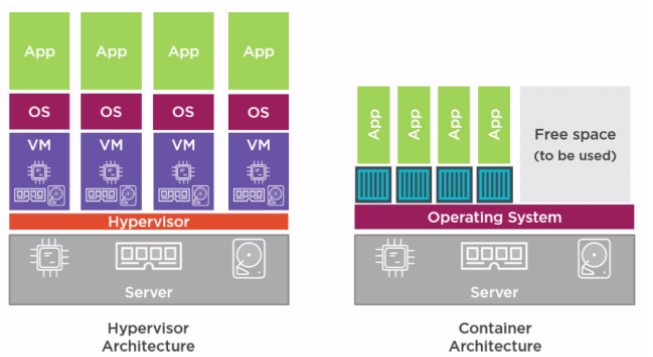
\includegraphics[scale=0.6]{\images/dockervsvirt.png}
        \caption{L'optimisation de docker par rapport à la machine }
        \label{fig:docker}
    \end{figure}
    \break

    \subsubsection{Tests}
    L'infrastructure est de devops .. plusieurs clusters 
    local / DEV / inté / prod , pour nous on s intéresse aux deux premières étapes. 

    Le but de ces tests et de tester la performance du cluster et son support de charge.

    \textbf{1er deploiement de test : le clustering avec HAProxy } :\\
    Communication entre les conteneurs en local avec minikube. 
    HAproxy est un load balancer pour les conteneurs docker
    Monitoring avec haproxy : outil intégré de visualiser le nbr de cnx , les instances ups
    \textbf{2eme deploiement de test : le clustering avec \gls{k8s} }\\
    Toutes les services et composants de CLoudNExt sont orchestrés par k8s.
    \gls{k8s} un  orchestrateur de conteneurs qui ... 
    un cluster de dev sur des machines réels hébergés à OVH. 
    l infrastructure est développé et maintenu par l'équipe serveur. 
    On trouve les composants de base toujours déployé et pour les nouveaux agents on les intégre en passant par helm.  

    Le but de ces tests et de tester la performance du cluster et son support de charge.
    **************************** les graphes de cnx *************************** \\

    Nombre de cnx par broker , par \\

    ************************ les graphes de percentile ***************************\\
    K8s traite la résilience \\

    Le monitoring se fait par InfluxDB/Grafana. Les composants remontent des métriques influxdb qui sont visibles par Grafana. 
        
    \subsubsection{Evaluation}

    Après avoir fini le développement et les tests de la première itération. 
    On évalue le système par rapport à nos exigences globaux du système. 
    Néanmoins lors de cette évaluation on est face à plusieurs problématiques qu il faut prendre en considération. 

    \begin{itemize}
        \renewcommand{\labelitemi}{$\bullet$}
        \item Le coût de communication sera élevé, car ça sera des paquets tcp dans des paquets MQTT 
        \item L'ajout du maintien d’un nouveau broker avec sa BD: ceci ajoute de la complexité à gérer.
        \item La manière de consommer depuis le broker: 
        \begin{itemize}
            \item \textbf{un seul consomateur gloabl :} \\
            \textbf{Avantages :} Lire tout du broker, Ecrire tous au clients sans avoir besoin de partager la consommation 
            sur plusieurs consommateurs. D'un autre coté, avec une telle manière de consommation on assure que tous les messages 
            sont toujours dans le broker jusqu'à leurs consommation lorsque la persistance est assuré par le broker MQTT\\
            \textbf{Inconvénients :} Problème de \textit{Single Point Of Failure} car si le consommateur tombe il y aura un blocage sur toute 
            la chaîne. Cette résilience peut être traité par \gls{k8s}, mais elle entraine une latence considérable si elle est réccurente. 
            \item \textbf{plusieurs consomatteurs connectés selon une hiérarchie de topics :} \\
            \textbf{Avantages :} Théoriquement c'est la solution standard du protocole MQTT d'avoir plusieurs consommateurs 
                    par brokeret donc la plus adéquate à utiliser. \\
            \textbf{Inconvénients :} Pour les clients il y a pas d'hiérarchie clair pour les clients. 
                    D'autre part, il y a une différence importante de nombre d asset par client chez \gls{mdi21} 
                    la diversité des clients de \gls{mdi} fait que il y a des individus qui ne possèdent que qlq boitiers 
                    en revanche d'autres clients comme constructeurs d automobile possèdents des milliers. De point de vue 
                    scalabilité cela fera un problème vue que le nombre de consommateurs augmentera selon les clients.
                    Ou bien au contraire qu'un seul client augmente sa commande que finalement un seul thread consommateur 
                    n'accepte plus de connexions.
            \item \textbf{plusieurs consomatteurs connectés aux instances, un consommateur par instance de broker}: \\
            \textbf{Avantages :} un des avantages \\
            \textbf{Inconvénients :} C'est le couplage fort entre le broker et son consommateurs et donc c 'est contre.\\
        \end{itemize}
    \end{itemize}


    Différentes manières pour effectuer la consommation : 

    Pour chaque manière on étudie les avantages et les inconvénients ... 



    \textbf{Synthèse :}
    Cette première itération nous a prouvé la limite de MQTT pour le projet MD30. Elle sert comme une étude 
    sur la faisabilité d'intégration du standard dans le projet.
    La question qui se pose est , quelles sont les fonctionnalités MQTT que MD30 exige par rapport aux 
    diverses fonctionnalités offertes par MQTT ? = > ils sont peu : 
    Ce que MD30 exige de tout cela n’est que le mécanisme des acks qui sont traités par les headers des messages MQTT. 
    Donc ajouter des bytes de plus comme étant un header dans le nouveau format de message du boîtier permet ce mécanisme. 
    => une implémentation fait-maison de ça fera l'affaire. \\




    \textbf{Conclusion} \break
            Après avoir fait une évaluation de la première itération et faire l étude de coût et performances de MQTT, 
        nous nous rendons compte que ce dernier est tellement riche en exigences divergente des exigences de MD30 et 
        donc l'adopter tel qu il comme le protocole de communication de MDI n’était pas la bonne solution. 


    



  

